\documentclass[letterpaper,10pt]{article}
\usepackage[margin=2cm]{geometry}

\usepackage{graphics}
\usepackage{xeCJK}

\setlength{\parskip}{1em}
\setlength{\parindent}{2em}
\usepackage{indentfirst}

\usepackage[colorlinks=true]{hyperref}

\renewcommand{\figurename}{图}

\title{\textbf{初来乍到CMU之生活小指南}}
\author{HMW-Alexander}

\begin{document}
	\maketitle
	
	签证被行政审查了21天后,终于在6月25号拿到了护照,然后匆匆抢到了27号(CST)飞往匹兹堡的最后一张机票。一切还算顺利,终于在学校规定的27号(EST)赶到了匹兹堡,开始了我的CMU生活。到今天,已经是整整一个月了,感觉时间飞逝,同时听闻秋季入学的同学们马上就要来了,于是记下一些东西\footnote{不过我也是菜鸟了,只写些觉得重要的事情和日常生活的一些小事。},分享给大家以做参考,希望新人们顺利开始自己的CMU生活。
		
	\section{入学需要办理的事情和流程}
	
	如何顺利开始正式的学校生活,应该是新人们来匹兹堡最关心的事情之一,这里就个人经历列出入学需要办理的事情和流程:
	
	\begin{figure}[!h]
		\centering
		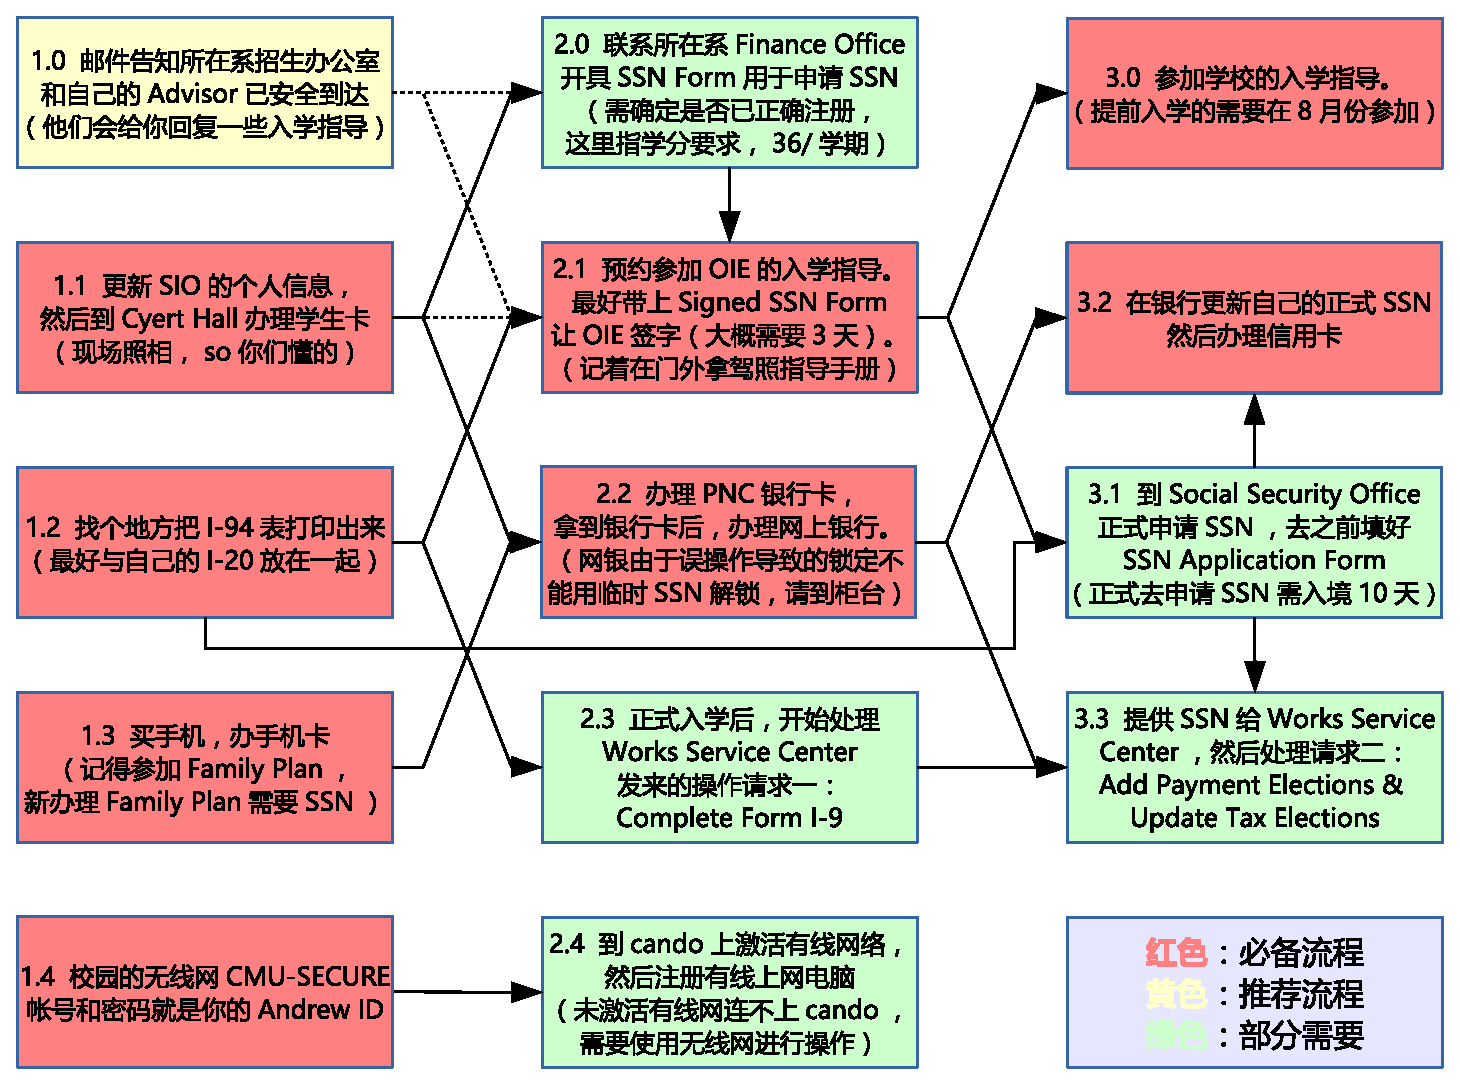
\includegraphics[width=0.8\textwidth]{./img/flowchart}
		\caption{一列里的项目编号没有优先度区分,有向实线链接表示必备前提要求关系。}
		\label{fig:flowchart}
	\end{figure}
	
	对于上述项目,下面将介绍一些小细节,请对应编号查找:
	
	\subsection*{\#1.1 办理学生卡}
	
	\begin{itemize}
		\item 需要到Cyert Hall办理(位置见图\ref{fig:cyert})。
		\item 进门直走,看到SIO之类的指示牌之后左转,走进去就到了。
		\item 第一次办卡不需要交钱。
		\item 现场照相(虽然我之前上传了照片,但是仍然让我现场照相)。
		\item 学生卡立等可取。
		\item 有了学生卡,你就可以坐校车,免费坐公交车(坐公交方法见2.1节)。
	\end{itemize}
	
	\begin{figure}[!h]
		\centering
		\includegraphics[width=0.8\textwidth]{./img/cyert}
		\caption{在Forbes和Morewood交叉口附近,黄色五星是入口所在处。}
		\label{fig:cyert}
	\end{figure}
	
	\subsection*{\#2.0 联系所在系Finance Office开具SSN Form}
	
	这里只对应ECE的同学,其他系的同学请询问你的Graduate Advisor(在offer letter上指定的有)。
	
	\begin{itemize}
		\item 联系ECE Finance Office(\url{ece-business@ece.cmu.edu})说明需要SSN Form(\url{http://www.cmu.edu/oie/SSNForm.pdf})
		\item 然后他们会回信让你在某个时间去Hamerschlag Hall(HH) 1110(进门直走左边)取SSN Form。
		\item 带上学生证,需要提供导师信息。
	\end{itemize}
	
	\subsection*{\#2.1 预约参加OIE的入学指导}
	
	这里由于我是提前入学,所以预约方式可能不同。
	
	\begin{itemize}
		\item 打电话(412-268-5231),或者到OIE办公室前台预约。前台在Warner Hall(图\ref{fig:warner})的三层,出电梯右手边,直接进门。预约会指定一位Advisor给你,然后准时去OIE办公室就可以了。
		\item 带上护照,I-20,I-94。
		\item 获得SSN Form的同学,可以将表给指定的Adisor。他需要检查你的注册情况,然后签字,一般要3天。注意,要获得OIE的签字,注册的时候,必须满足36学分/学期,否则不会给你签字(请联系你的Graduate Advisor解决该问题)。
		\item 离开OIE的时候,在门口有“Pennsylvania Driver's Manual”。可以自取又来考驾照的笔试。
	\end{itemize}
	
	\begin{figure}[!h]
		\centering
		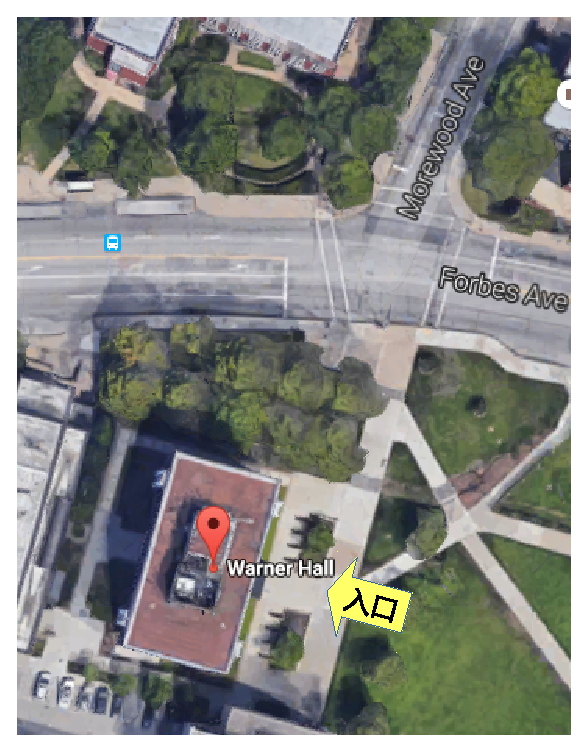
\includegraphics[width=0.3\textwidth]{./img/warner}
		\caption{在Forbes和Morewood交叉口附近,黄色箭头是入口所在处。}
		\label{fig:warner}
	\end{figure}
	
	\subsection*{\#2.2 办理PNC银行卡}
	
	\begin{itemize}
		\item 学校附近的PNC银行在Fifth和Craig的交叉口,周六上午也上班。
		\item 办理银行卡需要预约(图\ref{fig:pnc})。你可以到柜台预约,一般预约后第二天来办,也可以邮件预约(没试过)。
		\item 带上护照和学生证,开户需要往里面存少许钱(25刀?具体忘了)。
		\item 银行账户两个工作日激活,银行卡一到两周寄到你的邮箱。
		\item 收到银行卡后,需要按照银行卡上的标签打电话激活。
		\item 有了银行卡,就可以去办理网上银行。
		\item 随卡寄来的还有另一封邮件,是网上银行id,也是你的临时SSN,但这个不能用来解锁锁定的网上银行。
		\item 获得SSN后可以到PNC更新你的正式SSN。
	\end{itemize}
	
	\begin{figure}[!h]
		\centering
		\includegraphics[width=0.6\textwidth]{./img/pnc}
		\caption{在Fifth和Craig交叉口,黄色箭头是入口所在处。}
		\label{fig:pnc}
	\end{figure}
	
	\subsection*{\#2.3 Complete Form I-9}
	
	\begin{itemize}
		\item (ECE同学)在入学的时候,Michelle Echko (Finance Associate)会联系你,要求你尽快提供发工资的开始日期信息(stipend start date information),这个由你导师决定。
		\item 确定开始日期后,CMU Works Service Center就会给你的Andrew邮箱发操作指示。第一个就是填写I-9。
		\item 分三个步骤,其中第一二步骤需要自己在开始日期后三天内完成:
		\begin{enumerate}
			\item 在workday网上填表(入口:\url{https://www.cmu.edu/cmuworks/})
			\item 带上护照,I-20,I-94,学生卡去CMUWorks Service Center(图\ref{fig:works})的前台做认证。
		\end{enumerate}
		\item 进门需要刷学生卡。
		\item 之后他们需要你提交SSN,你申请到后去提交就可以了。
		\item 只有有了SSN,你才能绑定自己的银行卡领工资。
	\end{itemize}
	
	\begin{figure}[!h]
		\centering
		\includegraphics[width=0.5\textwidth]{./img/works}
		\caption{在Henry上,黄色箭头是入口所在处。}
		\label{fig:works}
	\end{figure}
	
	\subsection*{\#2.4 有线网络设置}
	
	\begin{itemize}
		\item 总配置流程见 \url{http://www.cmu.edu/computing/network/wired/}
		\item CANDO的配置流程见 \url{http://www.cmu.edu/computing/network/wired/cando.html}
		\item CANDO配置中需要提供网口编号,一般就在网口边上(图\ref{fig:outlet})
	\end{itemize}
	
	\begin{figure}[!h]
		\centering
		\includegraphics[width=0.2\textwidth,angle=-90]{./img/outlet}
		\caption{上面标签对应From,下面标签对应To}
		\label{fig:outlet}
	\end{figure}
	
	\subsection*{\#3.1 正式申请SSN}
	
	\begin{itemize}
		\item 申请SSN需要去Social Security Office。离CMU较近的有两个:
		\begin{itemize}
			\item East Liberty: 6117 Station Street (图\ref{fig:ssn})
			\item Downtown: 921 Penn Avenue
		\end{itemize}
		\item 工作时间是9:00到3:00(一、二、四、五)或12:00(三)
		\item 带上护照,I-94,I-20,SSN Form,Application Form(到那找到表,再填也可以)
		\item 流程很简单:
		\begin{itemize}
			\item 进门前台找到安全人员,说要申请SSN。
			\item 他会问你带武器没有,要求你手机静音,问你有没有预约,没有预约就去前台旁的领号机领号。
			\item 领完号就等着叫你,叫到你就把材料提供给他,然后就等着他把材料录入,最后返还给你所有材料。
			\item 完了之后就回家等把,SSN会寄到你的邮箱,一般一到两周。
		\end{itemize}
	\end{itemize}
	
	\begin{figure}[!h]
		\centering
		\includegraphics[width=0.6\textwidth]{./img/ssn}
		\caption{位于Centre和Station交叉口,黄色箭头是入口处所在。}
		\label{fig:ssn}
	\end{figure}
	
	\section{生活中那些鸡毛蒜皮的小事}
	
	\subsection{乘坐公交}
	
	\begin{figure}[!h]
		\centering
		\includegraphics[width=0.5\textwidth]{./img/onbus}
		\caption{【如何乘坐公交车】左图:公交车站牌是这个样子的,公交站一般在路口交通灯前方,大多以交叉路口命名,例如这处车站是Fifth Ave. at Craig,有71B/D,75路车。右图:车门处的刷卡机,使用校园卡每次乘车刷一次,一般上车时刷,但有时司机会把手捂住刷卡机,表明你需要下车的时候刷。}
	\end{figure}
	
	\begin{figure}[!h]
		\centering
		\includegraphics[width=0.8\textwidth]{./img/offbus}
		\caption{【如何下车】匹兹堡公交不是每站都停的,需要拉铃要求停车。左图:车前方顶部有LED屏幕显示下一站点名称,途中所示是Fifth @ Morewood,一般无语音报站,所以需要时刻关注。中图:当需要下车时,拉动黄色塑胶绳子,该绳子分布在公交车两侧窗框上,用来牵动前面的触发装置。右图:当拉下黄色塑胶绳子后,会响一声铃,报“stop requested”,同时LED屏幕显示“Stop\_reQuested”。}
	\end{figure}
	
	\subsection{吃饭给小费}
	
	流程如下(只以信用卡支付为例):
	\begin{itemize}
		\item 吃完饭后结帐(check)。
		\item 会给你一个账单,一般放在一个夹子或者盘子里。
		\item 然后你把信用卡放到夹子或者盘子里,他们拿走后刷卡。
		\item 之后会把一个付款单和信用卡一起放在同一个夹子或者盘子里送回来。
		\item 你需要在付款单上的小费栏(tips)上填写小费金额并签字,小费一般是消费额的10\%到20\%。
		\item 写完后,收好你的信用卡,把付款单留在夹子或者盘子里,你就可以走了。
	\end{itemize}
	
	\subsection{租车搬二手家具}
	
	\begin{figure}[!h]
		\centering
		\includegraphics[width=0.8\textwidth]{./img/renttruck}
		\caption{搬家一般从U-HAUL租一辆卡车,需要有驾照的人开车。费用包含租车费+里程+油钱,一般100刀以内搞定。卡车非常容易开,小女生也可以快速上手,一点问题都没有。}
	\end{figure}
	
	\begin{figure}[!ht]
		\centering
		\includegraphics[width=0.8\textwidth]{./img/kenmawr}
		\caption{住在Knemawr的同学往家里搬东西非常容易。在Howe Street有一个专门给卡车卸货的Dock(左图),此处的门(中图)需要从里面打开(也可以按门铃让doorman给你开),进门就是货梯(右图),空间非常大,电梯控制面板上面有一个switch用来锁定电梯门,在装卸过程中一定要扳成锁定状态,解除锁定电梯就可以动了。Kenmawr提供免费的cart用来搬运货物,非常方便。}
	\end{figure}
	
	\begin{figure}[!ht]
		\centering
		\includegraphics[width=0.8\textwidth]{./img/returntruck}
		\caption{左图:搬完东西后,在还车之前需要加油直到租车时的油量多一点(开回去还会耗掉一些油)。右图:U-HAUL晚上7点关门,之后还车的话,把车停到U-HAUL的停车场,把钥匙和合同塞进一个红色邮箱就可以了。}
	\end{figure}
	
\end{document}